\documentclass[11pt]{beamer}
\usepackage[utf8]{inputenc}
\usepackage[T1]{fontenc}
\usepackage{lmodern}
\usetheme{CambridgeUS}
\usepackage{graphicx}
\usepackage{hyperref}
\theoremstyle{boldstyle}
\newtheorem{proposition}[theorem]{Proposition}
\usepackage{tikz}
\usetikzlibrary{arrows.meta, positioning}
\begin{document}
	\author{Thomas D Jeitschko, Mark J Tremblay}
	\title{Platform Competition with Endogenous Homing}
	%\subtitle{}
	%\logo{}
	%\institute{}
	%\date{}
	%\subject{}
	%\setbeamercovered{transparent}
	%\setbeamertemplate{navigation symbols}{}
	\begin{frame}[plain]
		\maketitle
	\end{frame}
	
	\begin{frame}
		\frametitle{Introduction}
		\begin{itemize}
			\item \textbf{Platform:} Platform is basically an intermediary which facilitates interaction between two or more group of agents. That group can be buyer or seller. e.g., Amazon, Flipkart, Bumble, etc.
			
			\item \textbf{Homing:} Homing simply means agent subscribing to a platform. An agent can subscribe to a single Platform or Multiple Platforms. The graph below this illustrates this. 
		\end{itemize}
		\vspace{0.2cm}
	\begin{figure}[ht]
		\centering
	\begin{tikzpicture}[scale=0.5, transform shape, node distance=1.4cm]
		% Define nodes (users and platforms)
		\node (A) {User A};
		\node (B) [below=of A] {User B};
		\node (C) [below=of B] {User C};
		\node (D) [below=of C] {User D};
		
		\node (W) [right=3cm of A] {Platform W};
		\node (X) [right=3cm of B] {Platform X};
		\node (Y) [right=3cm of C] {Platform Y};
		\node (Z) [right=3cm of D] {Platform Z};
		
		% Draw connections
		\draw[-Latex] (A) -- (W);
		\draw[-Latex] (B) -- (Y);
		\draw[-Latex] (B) -- (Z);
		\draw[-Latex] (C) -- (W);
		\draw[-Latex] (C) -- (X);
		\draw[-Latex] (C) -- (Y);
		\draw[-Latex] (C) -- (Z);
		\draw[-Latex] (D) -- (Z);
	\end{tikzpicture}
	\end{figure}	
	\end{frame}
	
		\begin{frame}
		\frametitle{Introduction}
		Most of the literature has taken the bipartite graph as given, that is homing decisions are fixed prior to platforms deciding the price. In this paper, a two sided market is considered in which consumers and firm endogenously determine whether they single-home, multi-home or exit the market. \\
		\vspace{0.1cm}
		When exogenous homing decisions are assumed, allocation-specific pricing decisions occur. Exogenously fixed multi-homers face high prices as platforms do not compete for them(due to the fact that by assumption they join both the platforms), whereas exogenously fixed single-homers  face low prices.\\
		\vspace{0.1cm}
		\textbf{To understand how prices related to equilibrium homing decisions requires a model where platform set prices to endogenous homing decisions made by consumers and firm.}
		\end{frame}
		\begin{frame}
			\frametitle{The Model}
			\begin{small}
				
			
			\begin{itemize}
				\item Two group of agents on either side of the platforms (Consumers and Firms). 
				\item Agent on Side 1 are \textbf{Consumers} and Agent on Side 2 are called \textbf{Firms}.
				\item The benefits from interaction to an agent in one group depends on the number of agents of the other group.
				\item The platform charges each agent of the group a price to participate in the platform. 
				\item The model consider two platforms, $\mathbf{X} \in {\{A,B}\}$ .
				\item A multi-stage game. Simultaneous and non-cooperative actions.
				\item First, the platforms set prices to each of the two groups. 
				\item Thereafter, upon observing the platform prices, agents on each side, simultaneously make participation decisions. 
				\item Number of consumers that join \textbf{platform} $\mathbf{X-Y}$  is ${n_1}^\mathbf{x-y} \in {[0,\bar{N}_1]}$ and number of firms that join \textbf{platform} $\mathbf{X-Y}$ is ${n_2}^\mathbf{x-y} \in {[0,\bar{N}_2]}$ .
			\end{itemize}
		\end{small}
			
		\end{frame}
		
\begin{frame}
	\frametitle{The Model and Consumers}
	\begin{small}
		\begin{itemize}
			\item Cost to the platform of accommodating an agent on side $i \in \{1,2\}$ who joins platform is $f_i \geq 0$ and there are no fixed costs.
			\item The profit for platform $\mathbf{X}$ is given by $\prod^{\mathbf{X}}=n_1^{\mathbf{X}} (p_1^{\mathbf{X}}-f_1)+ n_2^{\mathbf{X}} (p_2^{\mathbf{X}}-f_2)$, where $p_i^{\mathbf{X}}$ is the uniform price that platform $\mathbf{X}$ charges to side $i$.
		\end{itemize}
		
		\vspace{0.1cm}
		\textbf{Side 1: Consumers}
		\begin{itemize}
			\item Consumers on side 1 draw their type $\theta_1$ from the distribution $F_1$ on support $[0,1]$.
			\item All consumers' outside option is valued at 0.
			\item Utility of consumer of type $\theta_1$ from single homing on platform $\mathbf{X}$ is given by $u_i^{\mathbf{X}}(\theta_1) = v+\alpha_1(\theta_1) n_2^{\mathbf{X}}- p_1^{\mathbf{X}}$ and $v \geq 0$
			\item Where $v$ is the membership benefits every consumer receives from joining the platform (received even if no firm joins). $v$ is type-independent and identical across platforms.
		\end{itemize}
	\end{small}	
\end{frame}
		
		\begin{frame}
			\frametitle{Consumers}
			\begin{small}
				\begin{itemize}
					\item  However, Consumers are heterogeneous in their marginal benefit from firms. 
					\item  The network effect (marginal benefit) to consumer of type $\theta_1$ for an additional firm on the platform is constant and given by $\alpha_1(\theta_1)$ also $\alpha_1(\theta_1) \geq 0$ . 
					\item $\alpha_1(\theta_1)$ is decreasing in $\theta_1$. That is, consumer whose $\theta_1$(type) is located far from zero have network effects (marginal benefit) higher relative to consumers whose $\theta_1$(type) is close to zero.
					\item We normalise $F_1$ to be uniform distribution over $[0,1]$ so that mass of type $\theta_1$ is given by $\theta_1. \bar{N}_1$ 
					\item The number of firms that join the platform $\mathbf{X}$ is $n_2^{\mathbf{X}}$.  
					\item There are two platforms, $A$ and $B$ , so consumer can join either one or both of them. In case of multi-homing, the utility of consumer is given by: $u_1^{\mathbf{M}}(\theta_1) = (1+\delta)v+\alpha_1(\theta_1).N_2-p_1^{A} - p_1^{B}$ 
				\end{itemize}
			\end{small}
		\end{frame}
		
		
				\begin{frame}
			\frametitle{Consumers }
			\begin{small}
				\begin{itemize}
					\item  Here, $N_2$ is the aggregate number of firms in Platform A and B. So, $n_2^A$ denotes number of firms joining platform A and $n_2^B$ denotes the number of firms joining platform B. Let $n_2^M$ be the number of firms multi-homing. Then, $N_2=n_1^A+n_2^B - n_2^M$. 
					\item  So having a firm available on both the platforms doesn't provide any extra benefits to the consumer. 
					\item Also, if a consumer joins two platforms, the intrinsic benefit from the second platform diminishes and hence the stand-alone marginal benefit is just $(1+\delta)v$ , $\delta \in [0,1]$. 
					
					
				\end{itemize}
			\end{small}
		\end{frame}
				
		\begin{frame}
			\frametitle{Firms }
			\begin{small}
				\begin{itemize}
					\item Firms on side 2 draw their type $\theta_2$ from the distribution $F_2$ on support $[0,1]$. Similar to side 1, we normalise $F_2$ to be uniform distribution over $[0,1]$, so that mass of type $\theta_2$ firms is given by $\theta_2.\bar{N}_2$  
					\item  All firm's outside option is 0. 
					\item Firm's payoff from single homing is given by, $u_2^{\mathbf{X}}(\theta_2)=\alpha_2(\theta_2).n_1^\mathbf{X} - c - p_2^\mathbf{X}$.
					\item Firms are heterogeneous in their marginal benefits from consumers. 
					\item The network effect(marginal benefit) to a consumer of type $\theta_2$ for an additional consumer on the platform is constant and given by $\alpha_2(\theta_2)$ .
					\item $\alpha_2(\theta_2)$ is decreasing in type $\theta_2$. That is, firms whose type $\theta_2$ is close to zero have marginal benefits that are high relative to those firms whose type is located far from zero. 
					
				\end{itemize}
			\end{small}
		\end{frame}
		
		\begin{frame}
	\frametitle{Firms }
	\begin{small}
		\begin{itemize}
			\item $p_2^\mathbf{X}$ is the price paid by the firm to platform $\mathbf{X}$.
			\item  Firm incur cost $c>0$ to join the platform. This cost reflects the cost of coding, programming, formatting their product to list in the platform, etc. 
			\item Firms are homogeneous with respect to their development and synchronisation cost.
			\item A firm which multi-homes has payoff, $u_2^M(\theta_2)=\alpha_2(\theta_2).N_1-(1+\sigma).c -p_2^A - p_2^B$ 
			\item Where $N_1= n_1^A+n_1^B-n_1^M$ , $n_1^A$ denotes number of consumer joining platform A, $n_2^B$ denotes number of firm joining platform B and $n_1^A$ denotes the number joining both the platforms. The firm only cares about number of distinct consumers present in the platforms. 
			\item  When a firm multi-homes, that is participate in two platforms, its synchronisation and development cost diminishes to $\sigma c$, with $\sigma \in [0,1]$ 
			
		\end{itemize}
	\end{small}
\end{frame}
	
		\begin{frame}
	\frametitle{Firms }
	\begin{small}
		\begin{itemize}
			\item Imagine the smartphone brand "Nothing" listing its product on both Amazon and Flipkart, now once a code has been written, with slight modification of the code, the same can be used in Flipkart too.  
			\item  The authors coins the term $\sigma$ representing the amount of "duplication economies" that exists when synchronising an app or game to a second platform.
			\item If $\sigma=1$, there exists no "duplication economies" and as $\sigma$ decreases, there exists "economies of duplication".
			
		\end{itemize}
	\end{small}
\end{frame}


		\begin{frame}
	\frametitle{Strategies and Equilibrium Concept}
	\begin{small}
		\begin{itemize}
			\item The paper focuses exclusively for Pure strategies and solves for the Subgame Perfect Nash Equilibrium . 
			\item  The authors exclusively focuses on prices  for which platforms have  not priced themselves out of the market. 
			\item The authors solve the game using backward induction. They first solve for how the allocation equilibrium would look like for different prices set by the platform and then they solve for equilibrium price for different allocation.
			\item They rule out the following equilibrium as it is trivial: The no-trade subgame equilibrium where no consumers and no firms join any platform is ruled out and off path, whenever there exists some equilibrium where some firms and consumers participate. 
			
			
		\end{itemize}
	\end{small}
\end{frame}


		\begin{frame}
	\frametitle{Strategies and Equilibrium Concept}
	\begin{small}
		\begin{itemize}

			\item 
			The authors make the following assumption: \textbf{If Platform Y has prices that are strictly better on one side of the platform and no worse on the other ($p_i^Y<p_i^X$ and $p_j^Y \geq p_j^X$ for $j \neq i$ ), then platform $Y$ has $n_k^Y > n_k^X$ for some $n=1,2$.} The authors preclude dis-coordinated allocation configurations in which despite having better (lower) prices, a platform fails to attract more agent than its rival on at least one side of the platform. The assumption says nothing about which side has greater participation. 
			
		\end{itemize}
	\end{small}
\end{frame}

\begin{frame}
	\frametitle{Equilibrium}
	Below is a summary of the equilibrium.
	\begin{figure}
		\centering
		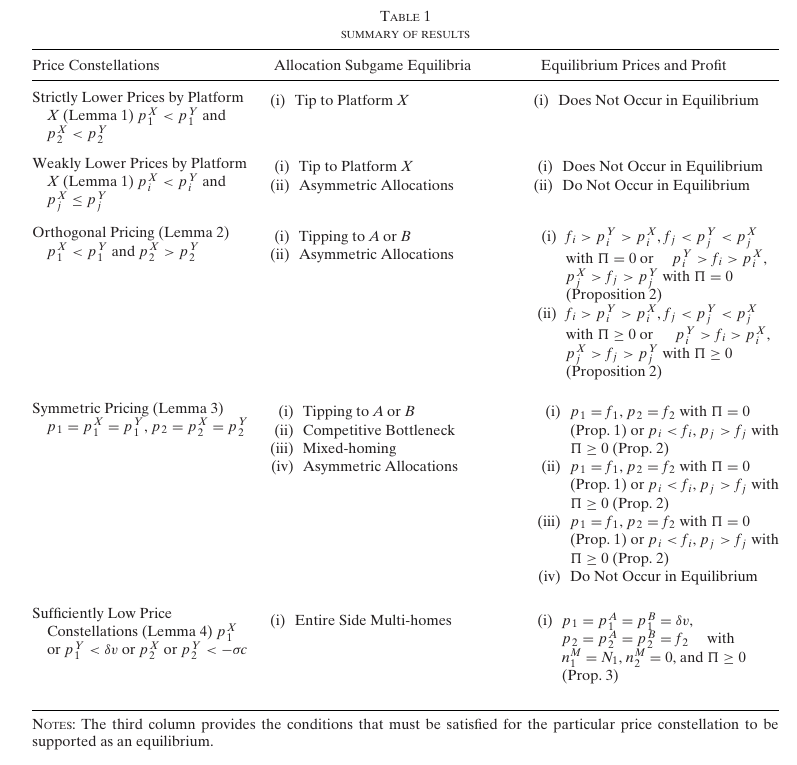
\includegraphics[width=0.6\linewidth]{eq.png}  % Simplified path
		\label{fig:equilibriumsummary}
	\end{figure}
\end{frame}

\begin{frame}
	\frametitle{Allocation equilibria for arbitrary prices}
	Authors define: $s_1=\delta v$ and $s_2=-\sigma c$ , so $s_i$ denotes the threshold utility for joining a second platform when that platform has no participation on other side of the market.\\
	
	In addition, let $w_1=\delta v + \alpha_1(0).\frac{\bar{N_2}}{2}>s_1$ and $w_2=-\sigma c + \alpha_1(0).\frac{\bar{N_1}}{2}>s_2$ , $w_i$ captures the maximum benefit to a side $i$ agent from joining a second platform when the platforms split participation equally on the other side of the market. 
	
	
\end{frame}
\begin{frame}
	\frametitle{Lemma 1}
	\begin{lemma}
		\textbf{(Allocations with a Lower Priced Platform):} Suppose that $s_i<p_i^X$ and $p_i^X \leq p_i^X$ for $i=1,2$ with at least one inequality being strict. If $p_i^Y<p_i^X$ for $i=1,2$ or if $p_i^Y<w_i<p_i^X$  and $p_j^Y=p_j^X$ for $i=1,2$ and $j\neq i$, then there exists a unique allocation equilibrium in which all active agents join Platform Y exclusively: $n_i^Y=N_i$ and $n_i^X=0$, for $i=1,2$. '
		> If $p_i^Y<p_i^X<w_i$  and $p_j^Y=p_j^X$ for $i=1,2$ and $j \neq i$, then tipping to platform Y is an equilibrium. In addition, there exists equilibrium allocations where all active Side $i$ agents multi-home $(n_i^X=n_i^Y=n_i^M)$ and the side $j$ agents single home so that $n_j^Y>n_j^X$
		
	\end{lemma}
	\begin{proof}
		Proof can be found  \href{https://shorturl.at/ZrOPF}{here}.
	\end{proof}
\end{frame}

\begin{frame}
	\frametitle{Lemma 1}
	\begin{itemize}
		\item Price undercutting by platform Y is successful as all agents tip to platform Y. With sufficiently low pricing on one side and prices equal on the other side, it is possible for the agents with low pricing to multihome(due to higher $\delta v, -\sigma c, \alpha_i(.)$) while the side for whom the prices are equal will single home in both X and Y, with higher number on platform Y. 
	\end{itemize}
\end{frame}

\begin{frame}
	\frametitle{Lemma 2}
	\begin{small}
	\begin{lemma}
\textbf{(Allocations Under Orthogonal Pricing):} When $p_1^A>p_1^B>s_1$ and $p_2^B>p_2^A>s_2$, there exists as many as three types of equilibria:
\begin{itemize}
	\item Tipping equilibria in which all active participation takes place on one platform. Tipping to platform B is always an equilibrium. A sufficient condition for tipping to platform A to be an equilibrium is that $p_1^Y>v$.
	\item There exists an equilibrium in which platform B only attracts multi-homing firms and platform A also attracts single homing firms, $n_2^M=n_2^B<n_2^X$, and high valued consumers single home on platform A, that is, $\theta_1 \in [0,\theta_1^A]$ where $n_1^A.\bar{N}_1$, and low valued consumers single-home on platform B, $\theta \in [\theta_1^A, \theta_1^* ]$ , where $N_1=\theta_1^*.\bar{N}_1$ and $n_1^B=N_1-n_1^A>n_1^A$. This allocation only exists when the consumer price difference is bounded and when the firm price difference is sufficiently large.
\end{itemize}
	
	\end{lemma}
\end{small}


\end{frame}

\begin{frame}
	\frametitle{Lemma 2}
	\begin{small}
	\begin{lemma}
		\textbf{(Allocations Under Orthogonal Pricing):} When $p_1^A>p_1^B>s_1$ and $p_2^B>p_2^A>s_2$, there exists as many as three types of equilibria:
		\begin{itemize}
			\item Similarly, for firm prices sufficiently close together, there exists an equilibrium in which platform A only attracts multi-homing consumers whereas Platform B also attracts single homing consumers, $n_1^M=n_1^A<n_1^B$; and high value firms single-home on Platform B, that is $\theta_2 \in [0,\theta_2^B]$, where $n_2^B=\theta_2^B\bar{N}_2$, and low-value firms single-home on Platform A, $\theta_2 \in [\theta_2^B, \theta_2^*]$, where $N_2=\theta_2^*\bar{N}_2$ and $n_2^B=N_2-n_2^B>n_2^B$. This allocation only exists when the firm price difference is bounded and $p_2^B>w_2$. 
		\end{itemize}
		
	\end{lemma}
	\begin{proof}
		Proof can be found  \href{https://shorturl.at/ZrOPF}{here}.
	\end{proof}
	\end{small}
\end{frame}

\begin{frame}
	\frametitle{Lemma 2}
	\begin{small}
\begin{itemize}
	\item For the first allocation, if All consumers tip to platform A, there's no incentive for any firm to either multi-home or distinctively join Platform B. The utility at platform A is the highest. Similar is the case, if all consumers and firms tip to platform B. None has any incentive to deviate. 
	\item In the second allocation, All active firms shift to platform A, while some does multi-homing at Platform B. There's no distinctive firm in Platform B. Consumers don't multi-home and does single-homing across both Platform A and Platform B. The high valued consumers single home at Platform A and low-valued consumers single-home on Platform B. The higher valued firms consumers pay a higher price $p_1^A$ in order to get access to large number of firms. The lower valued firms, pay less and gets access to lower number of forms.  This is only possible if there are large price difference across both the platforms and the price difference is bounded. If the price difference is too high, there's not much advantage for high valued consumers to join Platform A and if the price difference is too little, the low valued consumers will all shift to Platform A. 
\end{itemize}
	\end{small}
\end{frame}

\begin{frame}
	\frametitle{Lemma 2}
	\begin{small}
		\begin{itemize}
			\item The same argument goes for Allocation 3, just change consumer to firm and vice versa. 
			
		\end{itemize}
	\end{small}
\end{frame}

\begin{frame}
	\frametitle{Lemma 3}
	\begin{small}
		\begin{lemma}
			\textbf{(Allocations Under Symmetric Pricing):} When $p_1^A=p_1^B=p_1>s_1$ and $p_2^B=p_2^A=p_2>s_2$, there exists as many as three types of equilibria:
			\begin{itemize}
				\item Tipping equilibria in which all active participation takes place exclusively on one platform.
				\item Symmetric participation equilibria with $n_1^A=n_1^B=n_1$ and $n_2^A=n_2^B=n_2$.In a symmetric participation equilibrium, there exist multiple equilibrium allocations in which the distribution of multi-homers and single-homers on each side depends on the distribution of multi-homers and single-homers on the other side. The set of multi-homing consumers is given by $[0,n_1^M]$, and the set of single homing consumers are given by $(n_1^M,N_1]$. And the set of multi-homing firms is given by $[0,n_2^M]$, and the set of single-homing firms is given by $(n_2^M,N_2]$.
				\item Asymmetric participation equilibria can only exist when $p_i \leq w_i$. 
			\end{itemize}
			
		\end{lemma}
	\end{small}
\end{frame}

\begin{frame}
	\frametitle{Lemma 3}
	\begin{small}
	\begin{itemize}
		\item When platforms set equal prices, then an allocation where firms and consumers all tip to either of the one platform is an equilibria.
		\item There are multiple equilibria when there's equal split of firms on Platform A and B and there's equal split of Consumers on platform A and B. If consumer expects more firms to multi-home, then single homing becomes attractive for customers. If very less firms multi-homes, multi-homing becomes popular for customers. 
		Take and example of Flipkart and Amazon having 10 distinct seller each, same is with consumer side. Now, given similar prices, consumer will find it worthwhile to multi-home, as it will return them higher utility. 
		\item For the third allocation, depending on the price level, we will get the different asymmetry, like $n_1^A>n_1^B$ or $n_1^B>n_1^A$.  
	\end{itemize}
	\end{small}
\end{frame}

\begin{frame}
	\frametitle{Lemma 4}
	\begin{small}
		\begin{lemma}
			\textbf{(Prices Guranteeing Multi-Homing):} If $p_i^X,p_i^Y \leq s_i$ for $i=1,2$, then all agents multi-home in equilibrium. Similarly, if $p_i^X,p_i^Y \leq s_i$ and $p_j^Y \leq p_j^X$ with $p_j^X$ for $j \neq i$, then all side $i$ agents multi-home and all active side $j$ agents single-home on Platform Y so that $n_j^Y=N_j$ is an eqilibrium allocation; furthermore, if $p_j^Y=p_J^X$, then side $j$ agents are indifferent between the two platforms, since $p_j^Y-p_j^X$ and $n_i^X=n_i^Y=n_i^M$, and a continuum of single-homer distributions on side $j$ are possible in equilibrium. 

			
		\end{lemma}
	\end{small}
\end{frame}

\begin{frame}
	\frametitle{Lemma 4}
	\begin{small}
\begin{itemize}
	\item For the first case, where,$p_i^X,p_i^Y \leq s_i$ for $i=1,2$  All agents will multi-home cause by just joining the platform, we are getting positive utility. So all active agents would multi-home. 
	\item For the second case where, $p_1^X, p_1^Y \leq s_1$ and $p_2^Y \leq p_2^X$ , All consumers will multi-home while all firms will single-home on platform Y. In the case of equality in prices between two platforms for the firms, the firms will single-home either on Platform X or Y. 
	\item This completes the stage 2, SPNEs. Now, next the authors determine the equilibrium Price based on the allocations.  
\end{itemize}
	\end{small}
\end{frame}

\begin{frame}
	\frametitle{Proposition 1}
	\begin{small}
\begin{proposition}
	\textbf{(Strong Competition):}If $f_1>s_1$, then symmetric marginal cost pricing $(p_1=p_1^A=p_1^B=f_1)$ and $(p_2=p_2^A=p_2^B=f_2)$ with at least one and possibly three types of participation allocations occur in equilibrium:
	\begin{itemize}
		\item \textbf{(The competitive Bottleneck):}All active customers single-home and all active firms multi-home: $n_1^M=0, n_2^M=N_2$. This is always an equilibrium. 
		\item \textbf{(Mixed Homing):}A mix of multi-homing and single-homing consumers with multi-homing and single-homing firms: There exists $\bar{n}_1^M \in (0,N_1)$ so that ${n}_1^M \in (\bar{n}_1^M, N_1)$ and $n_2^M \in (0,N_2)$. Existence requires that $p_1<\delta v +\alpha_1(0)N_2$, where $N_2$ is given in Lemma 3.
		\item \textbf{(The inverse competitive bottleneck):} All active firms single-home and all active consumers multi-home: $n_1^M=n_1, n_2^M=0$. Existence requires that $p_1 \leq w_1$.
		\item In addition, tipping allocations also produce equilibria with symmetric marginal cost pricing.
	\end{itemize}
\end{proposition}
	\end{small}
\end{frame}

\begin{frame}
	\frametitle{Proposition 1}
	\begin{small}

			\begin{itemize}
				\item Successful price undercutting is not possible, when $f_i<s_i$ as seen by Lemma 4. So we need to have $f_1>s_1$. 
				\item And we consider symmetric marginal cost pricing, that is, $(p_1=p_1^A=p_1^B=f_1)$ and $(p_2=p_2^A=p_2^B=f_2)$. 
				\item Now any platform deviating to set a higher price means losing out all the customers(Lemma 1). 
				\item Such a move will wipe out higher priced platform from the market.
				\item  Lowering the pricing will cause the platform to earn negative profits. 
				\item So the allocations given in proposition 1 emerge as equilibrium allocations given the price mentioned in proposition. 
			\end{itemize}

	\end{small}
\end{frame}

\end{document}